\documentclass[11pt]{article}
\usepackage[margin=1in]{geometry}
\usepackage[T1]{fontenc}
\usepackage{lmodern,microtype}
\usepackage{booktabs,graphicx,amsmath,amssymb,hyperref,xcolor,enumitem,caption,float}
\usepackage[numbers,sort&compress]{natbib}
\hypersetup{colorlinks=true,linkcolor=blue!50!black,citecolor=blue!50!black,urlcolor=blue!50!black}
\captionsetup{font=small,labelfont=bf}
\setlist{nosep,leftmargin=1.4em}
\setlength{\parskip}{2pt}
\newcommand{\auroctestBone}{0.850}
\newcommand{\auroctestBoneLo}{0.803}
\newcommand{\auroctestBoneHi}{0.892}
\newcommand{\auprctestBone}{0.855}
\newcommand{\auprctestBoneLo}{0.810}
\newcommand{\auprctestBoneHi}{0.893}
\newcommand{\tprtestBone}{0.719}
\newcommand{\tprtestBoneLo}{0.648}
\newcommand{\tprtestBoneHi}{0.792}
\newcommand{\fprtestBone}{0.067}
\newcommand{\fprtestBoneLo}{0.040}
\newcommand{\fprtestBoneHi}{0.098}
\newcommand{\auroctestBtwo}{0.755}
\newcommand{\auroctestBtwoLo}{0.705}
\newcommand{\auroctestBtwoHi}{0.801}
\newcommand{\auprctestBtwo}{0.727}
\newcommand{\auprctestBtwoLo}{0.668}
\newcommand{\auprctestBtwoHi}{0.786}
\newcommand{\tprtestBtwo}{0.450}
\newcommand{\tprtestBtwoLo}{0.374}
\newcommand{\tprtestBtwoHi}{0.529}
\newcommand{\fprtestBtwo}{0.060}
\newcommand{\fprtestBtwoLo}{0.036}
\newcommand{\fprtestBtwoHi}{0.087}
\newcommand{\auroctestBthree}{0.839}
\newcommand{\auroctestBthreeLo}{0.793}
\newcommand{\auroctestBthreeHi}{0.885}
\newcommand{\auprctestBthree}{0.815}
\newcommand{\auprctestBthreeLo}{0.762}
\newcommand{\auprctestBthreeHi}{0.866}
\newcommand{\tprtestBthree}{0.556}
\newcommand{\tprtestBthreeLo}{0.475}
\newcommand{\tprtestBthreeHi}{0.631}
\newcommand{\fprtestBthree}{0.043}
\newcommand{\fprtestBthreeLo}{0.022}
\newcommand{\fprtestBthreeHi}{0.070}
\newcommand{\auroctestBtemp}{0.704}
\newcommand{\auroctestBtempLo}{0.643}
\newcommand{\auroctestBtempHi}{0.756}
\newcommand{\auprctestBtemp}{0.678}
\newcommand{\auprctestBtempLo}{0.610}
\newcommand{\auprctestBtempHi}{0.743}
\newcommand{\tprtestBtemp}{0.419}
\newcommand{\tprtestBtempLo}{0.339}
\newcommand{\tprtestBtempHi}{0.497}
\newcommand{\fprtestBtemp}{0.060}
\newcommand{\fprtestBtempLo}{0.035}
\newcommand{\fprtestBtempHi}{0.091}
\newcommand{\auroctestBnoprompt}{0.839}
\newcommand{\auroctestBnopromptLo}{0.793}
\newcommand{\auroctestBnopromptHi}{0.885}
\newcommand{\auprctestBnoprompt}{0.815}
\newcommand{\auprctestBnopromptLo}{0.762}
\newcommand{\auprctestBnopromptHi}{0.866}
\newcommand{\tprtestBnoprompt}{0.556}
\newcommand{\tprtestBnopromptLo}{0.475}
\newcommand{\tprtestBnopromptHi}{0.631}
\newcommand{\fprtestBnoprompt}{0.043}
\newcommand{\fprtestBnopromptLo}{0.022}
\newcommand{\fprtestBnopromptHi}{0.070}
\newcommand{\auroctestAPTG}{0.740}
\newcommand{\auroctestAPTGLo}{0.697}
\newcommand{\auroctestAPTGHi}{0.785}
\newcommand{\auprctestAPTG}{0.663}
\newcommand{\auprctestAPTGLo}{0.603}
\newcommand{\auprctestAPTGHi}{0.718}
\newcommand{\tprtestAPTG}{0.481}
\newcommand{\tprtestAPTGLo}{0.400}
\newcommand{\tprtestAPTGHi}{0.559}
\newcommand{\fprtestAPTG}{0.037}
\newcommand{\fprtestAPTGLo}{0.018}
\newcommand{\fprtestAPTGHi}{0.060}
\newcommand{\auroctestBfive}{0.564}
\newcommand{\auroctestBfiveLo}{0.509}
\newcommand{\auroctestBfiveHi}{0.617}
\newcommand{\auprctestBfive}{0.406}
\newcommand{\auprctestBfiveLo}{0.340}
\newcommand{\auprctestBfiveHi}{0.488}
\newcommand{\tprtestBfive}{0.106}
\newcommand{\tprtestBfiveLo}{0.062}
\newcommand{\tprtestBfiveHi}{0.155}
\newcommand{\fprtestBfive}{0.057}
\newcommand{\fprtestBfiveLo}{0.033}
\newcommand{\fprtestBfiveHi}{0.084}
\newcommand{\auroctestBsix}{0.418}
\newcommand{\auroctestBsixLo}{0.366}
\newcommand{\auroctestBsixHi}{0.468}
\newcommand{\auprctestBsix}{0.299}
\newcommand{\auprctestBsixLo}{0.256}
\newcommand{\auprctestBsixHi}{0.354}
\newcommand{\tprtestBsix}{0.025}
\newcommand{\tprtestBsixLo}{0.006}
\newcommand{\tprtestBsixHi}{0.053}
\newcommand{\fprtestBsix}{0.063}
\newcommand{\fprtestBsixLo}{0.038}
\newcommand{\fprtestBsixHi}{0.093}
\newcommand{\auroctestBeight}{0.737}
\newcommand{\auroctestBeightLo}{0.694}
\newcommand{\auroctestBeightHi}{0.781}
\newcommand{\auprctestBeight}{0.634}
\newcommand{\auprctestBeightLo}{0.567}
\newcommand{\auprctestBeightHi}{0.696}
\newcommand{\tprtestBeight}{0.362}
\newcommand{\tprtestBeightLo}{0.288}
\newcommand{\tprtestBeightHi}{0.441}
\newcommand{\fprtestBeight}{0.020}
\newcommand{\fprtestBeightLo}{0.007}
\newcommand{\fprtestBeightHi}{0.038}
\newcommand{\auroctestBnine}{0.864}
\newcommand{\auroctestBnineLo}{0.822}
\newcommand{\auroctestBnineHi}{0.904}
\newcommand{\auprctestBnine}{0.842}
\newcommand{\auprctestBnineLo}{0.797}
\newcommand{\auprctestBnineHi}{0.883}
\newcommand{\tprtestBnine}{0.631}
\newcommand{\tprtestBnineLo}{0.552}
\newcommand{\tprtestBnineHi}{0.708}
\newcommand{\fprtestBnine}{0.070}
\newcommand{\fprtestBnineLo}{0.042}
\newcommand{\fprtestBnineHi}{0.101}
\newcommand{\aurocoodBone}{0.873}
\newcommand{\aurocoodBoneLo}{0.813}
\newcommand{\aurocoodBoneHi}{0.924}
\newcommand{\auprcoodBone}{0.869}
\newcommand{\auprcoodBoneLo}{0.804}
\newcommand{\auprcoodBoneHi}{0.920}
\newcommand{\tproodBone}{0.725}
\newcommand{\tproodBoneLo}{0.630}
\newcommand{\tproodBoneHi}{0.822}
\newcommand{\fproodBone}{0.073}
\newcommand{\fproodBoneLo}{0.034}
\newcommand{\fproodBoneHi}{0.116}
\newcommand{\aurocoodBtwo}{0.787}
\newcommand{\aurocoodBtwoLo}{0.720}
\newcommand{\aurocoodBtwoHi}{0.844}
\newcommand{\auprcoodBtwo}{0.722}
\newcommand{\auprcoodBtwoLo}{0.626}
\newcommand{\auprcoodBtwoHi}{0.806}
\newcommand{\tproodBtwo}{0.375}
\newcommand{\tproodBtwoLo}{0.266}
\newcommand{\tproodBtwoHi}{0.479}
\newcommand{\fproodBtwo}{0.053}
\newcommand{\fproodBtwoLo}{0.020}
\newcommand{\fproodBtwoHi}{0.092}
\newcommand{\aurocoodBthree}{0.873}
\newcommand{\aurocoodBthreeLo}{0.813}
\newcommand{\aurocoodBthreeHi}{0.925}
\newcommand{\auprcoodBthree}{0.842}
\newcommand{\auprcoodBthreeLo}{0.765}
\newcommand{\auprcoodBthreeHi}{0.904}
\newcommand{\tproodBthree}{0.588}
\newcommand{\tproodBthreeLo}{0.481}
\newcommand{\tproodBthreeHi}{0.701}
\newcommand{\fproodBthree}{0.053}
\newcommand{\fproodBthreeLo}{0.019}
\newcommand{\fproodBthreeHi}{0.090}
\newcommand{\aurocoodBtemp}{0.763}
\newcommand{\aurocoodBtempLo}{0.686}
\newcommand{\aurocoodBtempHi}{0.832}
\newcommand{\auprcoodBtemp}{0.735}
\newcommand{\auprcoodBtempLo}{0.636}
\newcommand{\auprcoodBtempHi}{0.816}
\newcommand{\tproodBtemp}{0.512}
\newcommand{\tproodBtempLo}{0.400}
\newcommand{\tproodBtempHi}{0.623}
\newcommand{\fproodBtemp}{0.087}
\newcommand{\fproodBtempLo}{0.041}
\newcommand{\fproodBtempHi}{0.133}
\newcommand{\aurocoodBnoprompt}{0.873}
\newcommand{\aurocoodBnopromptLo}{0.813}
\newcommand{\aurocoodBnopromptHi}{0.925}
\newcommand{\auprcoodBnoprompt}{0.842}
\newcommand{\auprcoodBnopromptLo}{0.765}
\newcommand{\auprcoodBnopromptHi}{0.904}
\newcommand{\tproodBnoprompt}{0.588}
\newcommand{\tproodBnopromptLo}{0.481}
\newcommand{\tproodBnopromptHi}{0.701}
\newcommand{\fproodBnoprompt}{0.053}
\newcommand{\fproodBnopromptLo}{0.019}
\newcommand{\fproodBnopromptHi}{0.090}
\newcommand{\aurocoodAPTG}{0.762}
\newcommand{\aurocoodAPTGLo}{0.702}
\newcommand{\aurocoodAPTGHi}{0.822}
\newcommand{\auprcoodAPTG}{0.693}
\newcommand{\auprcoodAPTGLo}{0.603}
\newcommand{\auprcoodAPTGHi}{0.772}
\newcommand{\tproodAPTG}{0.550}
\newcommand{\tproodAPTGLo}{0.438}
\newcommand{\tproodAPTGHi}{0.662}
\newcommand{\fproodAPTG}{0.053}
\newcommand{\fproodAPTGLo}{0.019}
\newcommand{\fproodAPTGHi}{0.091}
\newcommand{\aurocoodBfive}{0.543}
\newcommand{\aurocoodBfiveLo}{0.461}
\newcommand{\aurocoodBfiveHi}{0.620}
\newcommand{\auprcoodBfive}{0.407}
\newcommand{\auprcoodBfiveLo}{0.315}
\newcommand{\auprcoodBfiveHi}{0.508}
\newcommand{\tproodBfive}{0.138}
\newcommand{\tproodBfiveLo}{0.062}
\newcommand{\tproodBfiveHi}{0.216}
\newcommand{\fproodBfive}{0.087}
\newcommand{\fproodBfiveLo}{0.044}
\newcommand{\fproodBfiveHi}{0.134}
\newcommand{\aurocoodBsix}{0.345}
\newcommand{\aurocoodBsixLo}{0.274}
\newcommand{\aurocoodBsixHi}{0.415}
\newcommand{\auprcoodBsix}{0.294}
\newcommand{\auprcoodBsixLo}{0.230}
\newcommand{\auprcoodBsixHi}{0.375}
\newcommand{\tproodBsix}{0.450}
\newcommand{\tproodBsixLo}{0.346}
\newcommand{\tproodBsixHi}{0.561}
\newcommand{\fproodBsix}{0.680}
\newcommand{\fproodBsixLo}{0.599}
\newcommand{\fproodBsixHi}{0.752}
\newcommand{\aurocoodBeight}{0.759}
\newcommand{\aurocoodBeightLo}{0.700}
\newcommand{\aurocoodBeightHi}{0.818}
\newcommand{\auprcoodBeight}{0.669}
\newcommand{\auprcoodBeightLo}{0.573}
\newcommand{\auprcoodBeightHi}{0.754}
\newcommand{\tproodBeight}{0.425}
\newcommand{\tproodBeightLo}{0.319}
\newcommand{\tproodBeightHi}{0.525}
\newcommand{\fproodBeight}{0.013}
\newcommand{\fproodBeightLo}{0.000}
\newcommand{\fproodBeightHi}{0.036}
\newcommand{\aurocoodBnine}{0.868}
\newcommand{\aurocoodBnineLo}{0.806}
\newcommand{\aurocoodBnineHi}{0.921}
\newcommand{\auprcoodBnine}{0.841}
\newcommand{\auprcoodBnineLo}{0.762}
\newcommand{\auprcoodBnineHi}{0.905}
\newcommand{\tproodBnine}{0.637}
\newcommand{\tproodBnineLo}{0.529}
\newcommand{\tproodBnineHi}{0.750}
\newcommand{\fproodBnine}{0.047}
\newcommand{\fproodBnineLo}{0.015}
\newcommand{\fproodBnineHi}{0.084}
\newcommand{\nEptrain}{230}
\newcommand{\nEpval}{276}
\newcommand{\nEptest}{460}
\newcommand{\nEpood}{230}
\newcommand{\nPosTest}{160}
\newcommand{\nTest}{460}
\newcommand{\nPosOod}{80}
\newcommand{\nOod}{230}
\newcommand{\dAurocBthreeBtwo}{0.084}
\newcommand{\dAurocBthreeBtwoLo}{0.031}
\newcommand{\dAurocBthreeBtwoHi}{0.139}
\newcommand{\dTprBthreeBtwo}{0.106}
\newcommand{\dTprBthreeBtwoLo}{0.018}
\newcommand{\dTprBthreeBtwoHi}{0.197}
\newcommand{\dAurocBthreeBone}{-0.011}
\newcommand{\dAurocBthreeBoneLo}{-0.077}
\newcommand{\dAurocBthreeBoneHi}{0.057}
\newcommand{\dTprBthreeBone}{-0.162}
\newcommand{\dTprBthreeBoneLo}{-0.267}
\newcommand{\dTprBthreeBoneHi}{-0.060}
\newcommand{\dAurocAPTGBthree}{-0.099}
\newcommand{\dAurocAPTGBthreeLo}{-0.138}
\newcommand{\dAurocAPTGBthreeHi}{-0.058}
\newcommand{\dTprAPTGBthree}{-0.075}
\newcommand{\dTprAPTGBthreeLo}{-0.130}
\newcommand{\dTprAPTGBthreeHi}{-0.029}
\newcommand{\dAurocAPTGBtwo}{-0.015}
\newcommand{\dAurocAPTGBtwoLo}{-0.074}
\newcommand{\dAurocAPTGBtwoHi}{0.045}
\newcommand{\dTprAPTGBtwo}{0.031}
\newcommand{\dTprAPTGBtwoLo}{-0.059}
\newcommand{\dTprAPTGBtwoHi}{0.122}
\newcommand{\dAurocBtempBtwo}{-0.051}
\newcommand{\dAurocBtempBtwoLo}{-0.124}
\newcommand{\dAurocBtempBtwoHi}{0.024}
\newcommand{\dTprBtempBtwo}{-0.031}
\newcommand{\dTprBtempBtwoLo}{-0.150}
\newcommand{\dTprBtempBtwoHi}{0.084}
\newcommand{\dAurocAPTGBone}{-0.110}
\newcommand{\dAurocAPTGBoneLo}{-0.175}
\newcommand{\dAurocAPTGBoneHi}{-0.040}
\newcommand{\dTprAPTGBone}{-0.237}
\newcommand{\dTprAPTGBoneLo}{-0.344}
\newcommand{\dTprAPTGBoneHi}{-0.129}
\newcommand{\dAurocBnineAPTG}{0.124}
\newcommand{\dAurocBnineAPTGLo}{0.084}
\newcommand{\dAurocBnineAPTGHi}{0.161}
\newcommand{\dTprBnineAPTG}{0.150}
\newcommand{\dTprBnineAPTGLo}{0.095}
\newcommand{\dTprBnineAPTGHi}{0.215}
\newcommand{\bEightPos}{0.36}
\newcommand{\bEightNeg}{0.02}
\newcommand{\bEightStop}{2}
\newcommand{\pilotNCZero}{6}
\newcommand{\pilotMeanCZeroSeatZero}{0.93}
\newcommand{\pilotMeanCZeroSeatOne}{0.78}
\newcommand{\pilotMeanCZeroSeatTwo}{0.78}
\newcommand{\pilotNCOne}{6}
\newcommand{\pilotMeanCOneSeatZero}{1.97}
\newcommand{\pilotMeanCOneSeatOne}{0.57}
\newcommand{\pilotMeanCOneSeatTwo}{0.45}
\newcommand{\pilotNCThree}{6}
\newcommand{\pilotMeanCThreeSeatZero}{4.00}
\newcommand{\pilotMeanCThreeSeatOne}{4.00}
\newcommand{\pilotMeanCThreeSeatTwo}{4.00}
\newcommand{\pilotNCFourL}{6}
\newcommand{\pilotMeanCFourLSeatZero}{2.68}
\newcommand{\pilotMeanCFourLSeatOne}{2.82}
\newcommand{\pilotMeanCFourLSeatTwo}{1.88}
\newcommand{\pilotCoordMean}{2.75}
\newcommand{\pilotCleanMean}{0.86}
\newcommand{\pilotMWp}{0.002}
\newcommand{\pilotInvalid}{0}
\newcommand{\pilotDecisions}{720}
\newcommand{\pilotCOnePertMean}{1.97}
\newcommand{\pilotCOnePartnerMean}{0.57}
\newcommand{\rlThrvaltpr}{0.81}
\newcommand{\rlThrvalfpr}{0.04}
\newcommand{\rlThrvaldelay}{40.0}
\newcommand{\rlThrvalcost}{3.00}
\newcommand{\rlThrtesttpr}{0.47}
\newcommand{\rlThrtestfpr}{0.03}
\newcommand{\rlThrtestdelay}{40.0}
\newcommand{\rlThrtestcost}{3.00}
\newcommand{\rlThroodtpr}{0.54}
\newcommand{\rlThroodfpr}{0.05}
\newcommand{\rlThrooddelay}{40.0}
\newcommand{\rlThroodcost}{3.00}
\newcommand{\rlSprtvaltpr}{0.42}
\newcommand{\rlSprtvalfpr}{0.02}
\newcommand{\rlSprtvaldelay}{33.8}
\newcommand{\rlSprtvalcost}{2.91}
\newcommand{\rlSprttesttpr}{0.36}
\newcommand{\rlSprttestfpr}{0.02}
\newcommand{\rlSprttestdelay}{32.1}
\newcommand{\rlSprttestcost}{2.89}
\newcommand{\rlSprtoodtpr}{0.42}
\newcommand{\rlSprtoodfpr}{0.01}
\newcommand{\rlSprtooddelay}{31.8}
\newcommand{\rlSprtoodcost}{2.87}
\newcommand{\rlUncvaltpr}{0.56}
\newcommand{\rlUncvalfpr}{0.02}
\newcommand{\rlUncvaldelay}{20.0}
\newcommand{\rlUncvalcost}{3.42}
\newcommand{\rlUnctesttpr}{0.37}
\newcommand{\rlUnctestfpr}{0.03}
\newcommand{\rlUnctestdelay}{20.0}
\newcommand{\rlUnctestcost}{3.27}
\newcommand{\rlUncoodtpr}{0.46}
\newcommand{\rlUncoodfpr}{0.05}
\newcommand{\rlUncooddelay}{20.0}
\newcommand{\rlUncoodcost}{3.26}
\newcommand{\rlSelCFP}{1}
\newcommand{\rlSelCObs}{0.05}
\newcommand{\rlPpovaltpr}{0.33}
\newcommand{\rlPpovaltprSd}{0.00}
\newcommand{\rlPpovalfpr}{0.02}
\newcommand{\rlPpovalfprSd}{0.00}
\newcommand{\rlPpovaldelay}{20.0}
\newcommand{\rlPpovaldelaySd}{0.0}
\newcommand{\rlPpovalcost}{1.00}
\newcommand{\rlPpovalcostSd}{0.00}
\newcommand{\rlPpotesttpr}{0.37}
\newcommand{\rlPpotesttprSd}{0.00}
\newcommand{\rlPpotestfpr}{0.03}
\newcommand{\rlPpotestfprSd}{0.00}
\newcommand{\rlPpotestdelay}{20.0}
\newcommand{\rlPpotestdelaySd}{0.0}
\newcommand{\rlPpotestcost}{1.00}
\newcommand{\rlPpotestcostSd}{0.00}
\newcommand{\rlPpooodtpr}{0.46}
\newcommand{\rlPpooodtprSd}{0.00}
\newcommand{\rlPpooodfpr}{0.05}
\newcommand{\rlPpooodfprSd}{0.00}
\newcommand{\rlPpoooddelay}{20.0}
\newcommand{\rlPpoooddelaySd}{0.0}
\newcommand{\rlPpooodcost}{1.00}
\newcommand{\rlPpooodcostSd}{0.00}
\newcommand{\rlMatched}{reached}
\newcommand{\rlFwvaltpr}{0.33}
\newcommand{\rlFwvalfpr}{0.02}
\newcommand{\rlFwtesttpr}{0.37}
\newcommand{\rlFwtestfpr}{0.03}
\newcommand{\rlFwoodtpr}{0.46}
\newcommand{\rlFwoodfpr}{0.05}
\newcommand{\rlFwDiff}{-0.106}
\newcommand{\rlFwDiffLo}{-0.158}
\newcommand{\rlFwDiffHi}{-0.053}
\newcommand{\rlNeverAlertCfgs}{3}

\newcommand{\gij}{g_{i\to j}}
\title{\vspace{-1.2em}Each Dependence Statistic Covers a Different Set of Collusion Mechanisms:\\ A Pre-Registered, Sprint-Scale Test of Directional Predictive Gain (APTG-RL)}
\author{Aravinth K\\ Independent researcher \quad \texttt{aravinth3007k@gmail.com}\\[2pt] \textit{With Apart Research}}
\date{}
\begin{document}
\maketitle
\thispagestyle{empty}
\begin{abstract}\small\noindent
Collusion audits must tell coordination apart from shared context, shared models and prompt-induced shifts. We test the APTG-RL design: a directional predictive-gain statistic between agents, a time-varying directed graph with temporal features, and a reinforcement-learning investigator that decides when to alert (its prompt-conditioned baseline is not exercised by the reported detectors). We build a three-seller repeated pricing game with four scripted collusion mechanisms, benign and shared-model negatives, and seven conditions (C0--C6) of unilateral and common perturbations, collusion and benign shifts. Ten detectors are compared on held-out episodes at validation-fixed thresholds under a pre-registered plan. Pre-registered H1 (directional beats both symmetric MI and net influence) is not supported: a combined same-round-and-lagged gain beats symmetric MI (AUROC \auroctestBthree{} vs.\ \auroctestBtwo{}) but has significantly lower TPR than lag-1 net influence (\dTprBthreeBone{}; AUROC \auroctestBone{}); its strictly lagged part alone showed no clear advantage over symmetric MI (AUROC \auroctestBtemp{} vs.\ \auroctestBtwo{}; difference inconclusive), and the parametric gain misses a parity-coded hidden channel that mutual information catches. The temporal-graph score did not help (\auroctestAPTG{}), and the RL investigator only rediscovered a ``look at the first window'' rule, trading recall for lower delay and cost. An exploratory follow-up union (max-$z$) of net influence, symmetric MI and directional gain covers all four mechanisms (AUROC 0.990; TPR 0.95). No statistically clear increase in false alarms was established under unilateral instruction perturbation, although small condition-level samples leave moderate increases possible. A small Claude Haiku~4.5 pilot (\pilotDecisions{} decisions, \pilotInvalid{} invalid) confirms the perturbation shifts behaviour. Evidence is simulator-only and small-scale; we report nulls, deviations and limits.
\end{abstract}

\section{Introduction}
Multi-agent LLM systems can coordinate through explicit messages, response patterns, complementary actions or hidden channels. Two independent agents can also look coordinated because they share a prompt, a task state or a base model, and an instruction given to only one agent can change that agent's behaviour without any collusion. A useful auditor must therefore ask whether one agent's history carries \emph{extra, directional} information about another's next action beyond context, own history and prompt condition, and must do so without raising false alarms when only one agent has been steered.

We implement the APTG-RL design (our own research proposal, written before the sprint) and evaluate it on a controlled testbed, with one caveat stated up front: its prompt-conditioned baseline is implemented and unit-tested but is not used by the reported detectors (Section~5), so the prompt-conditioning hypothesis is not tested. Our contributions are:
\begin{enumerate}
\item \textbf{A controlled collusion-audit testbed.} A 3-seller repeated pricing game, four scripted collusion mechanisms (complementary, leader--follower, alternating, hidden-channel), three non-collusive controls (independent, shared-model, benign adaptation), and a seven-condition controlled experimental design (C0--C6) covering unilateral and common instruction perturbations, scripted collusion, collusion under perturbation and benign policy shifts, with held-out mechanisms and a held-out prompt family.
\item \textbf{A pre-registered comparison of ten detectors}, including directional predictive gain, a windowed directed-graph score, an RL investigator and the information-theoretic baseline of Bonjour et al., with episode-level bootstrap CIs, plus a log of every deviation from the plan.
\item \textbf{Findings, including nulls.} A combined same-round-and-lagged gain beats symmetric MI but not lag-1 MI, and its strictly lagged part alone shows no clear advantage over symmetric MI; each statistic is mechanism-specific and the set is complementary; the graph score and RL investigator did not add value at this scale; no detector showed a clear false-alarm rise under unilateral perturbation; and an exploratory max-$z$ union of net influence, symmetric MI and directional gain covers all four mechanisms (AUROC 0.990 against 0.850 for the best single statistic). We make no priority claim.
\end{enumerate}

\section{Related Work}
\textbf{Information-theoretic detection.} Bonjour et al.~\cite{bonjour2022} use mutual information between agents' actions to detect covert cooperation in repeated games; we implement a net-influence variant as baseline B1 and a symmetric-MI variant as B2. Our directional statistic is the held-out predictive-gain analogue of transfer entropy~\cite{schreiber2000} and Granger-style prediction~\cite{granger1969}.
\textbf{LLM collusion.} Motwani et al.~\cite{motwani2024} formalise secret collusion via steganography; Mathew et al.~\cite{mathew2025} study the emergence and mitigation of steganographic collusion; Colosseum~\cite{nakamura2026} audits collusion in cooperative multi-agent systems using objective-based regret and separates attempted from effective collusion; Rose et al.~\cite{rose2026} detect collusion from model activations (white-box, which we do not use).
\textbf{Graphs and sequential sensing.} Eschenbaum and Meylahn~\cite{eschenbaum2026} audit pricing algorithms from static strategy graphs; Joseph et al.~\cite{joseph2024} cast anomaly detection with observation costs as sequential controlled sensing with learned policies. We use dynamic interaction graphs from trajectories and a sensing-style investigator.
\textbf{Behaviour is prompt- and endpoint-conditioned.} Work on LLM behavioural fingerprinting and endpoint stability~\cite{leshin2026,hu2026} is adjacent motivation for treating an agent's output distribution as dependent on prompts, endpoints and configurations (the premise behind the C1/C2/C6 controls); it does not validate a prompt-conditioned collusion detector, and our prompt-conditioned baseline remains untested here.

\section{Methods}
\textbf{Environment.} Three sellers play $T{=}40$ rounds; each chooses a price level $a\in\{0,\dots,4\}$; the lowest price takes the market (ties split) and the payoff is price$\times$share. Agents $\{0,1\}$ are the candidate coalition, agent~2 is an outsider. Non-collusive base policies are categorical, with prompt-family and severity shifts, own-action stickiness and a weak coupling to public lagged prices.
\textbf{Mechanisms.} \emph{Complementary}: $b_t=4-a_t$ w.p.\ 0.8. \emph{Leader--follower}: $b_t=a_{t-1}$ w.p.\ 0.8. \emph{Alternating}: turn-taking. \emph{Hidden-channel}: the parity of $a_t$ shifts $b_{t+1}$ (a closed toy protocol). Negatives: independent, shared-model, and benign adaptation (both respond to the outsider, never to each other).
\textbf{Conditions.} C0 clean; C1/C2 a perturbation of agent~0/1 only; C3 a common perturbation; C4 scripted collusion; C5 collusion plus a unilateral perturbation; C6 a benign policy shift in one agent. Splits are by whole episode: train seeds 0--9, validation 50--61, test 75--94, and OOD 100--109 using a prompt family never seen in calibration; \emph{alternating} and \emph{hidden-channel} are excluded from every labelled fit (\dag{} in tables); only B9 and the RL investigator are fit on labelled episodes, so the hold-out constrains them and not the unsupervised detectors, whose design (linear model, lags 0--2) we chose knowing the mechanisms. Cells have \nEpval{}/\nEptest{}/\nEpood{} validation/test/OOD episodes in total.
\textbf{Directional gain.} For an ordered pair, a regularised multinomial logistic model of $a_j^t$ on its own lag and the public lag of the third agent (prompt covariates in both models, which are constant within an episode and therefore inert) is compared with the same model plus a set $L$ of the source agent's lags (lag 0 is the source's action in the \emph{same} round), on contiguous held-out folds:
\[ g^{(L)}_{i\to j}=\tfrac1N\textstyle\sum_t\big[\log p_1(a^t_j\mid\cdot,H_i)-\log p_0(a^t_j\mid\cdot)\big]. \]
\textbf{Two kinds of evidence.} Because sellers move simultaneously, $L{=}\{0,1,2\}$ (B3) mixes \emph{contemporaneous} dependence, $S_{ij}=I(A_i^t;A_j^t\mid X)$, which sees same-round relations such as complementary pricing ($b_t=4-a_t$), with \emph{lagged} predictive gain from lags $1,2$ (B3-temporal, the strictly directional statistic $G_{i\to j}$, whose comparison with $G_{j\to i}$ reveals direction). We keep the pre-registered B3 as a \emph{combined} score and report $G_{i\to j}$ separately.\\[2pt]\textbf{Population interpretation.} Let $Y=a_j^t$, $X$ the conditioning variables (target's own history, the third agent's public lag, prompt covariates) and $Z$ the source's lag set. If $p_0(y\mid x)=P(Y{=}y\mid X{=}x)$ and $p_1(y\mid x,z)=P(Y{=}y\mid X{=}x,Z{=}z)$ are the true conditionals, then\[ \mathbb{E}\!\left[\log\frac{p_1(Y\mid X,Z)}{p_0(Y\mid X)}\right]=I(Y;Z\mid X)=\mathbb{E}_{X,Z}\,D_{\mathrm{KL}}\!\big(P(Y\mid X,Z)\,\|\,P(Y\mid X)\big)\ge 0, \]so the population gain is the extra information $Z$ carries about $Y$ beyond $X$. This is an identity under correct specification, not a result about collusion. Held-out estimates can be negative (estimation error, sampling variability), and with a misspecified model class they measure the gain \emph{of that class}, which is why a logistic model on numeric lags misses a parity code. The gain is predictive, not causal: omitted common causes, public feedback and shared environmental information also produce it, so a significant edge is evidence of dependence under the stated conditioning set, not proof of collusion.\\[2pt]B3 ($L{=}\{0,1,2\}$) is $\max_{i\neq j}$ of the robust $z=(g-\mathrm{med}\,G_0)/(1.4826\,\mathrm{MAD}\,G_0)$ against gains from clean training negatives; B3-temporal uses $L{=}\{1,2\}$ only; B3-noprompt drops prompt covariates.
\textbf{Graph (APTG).} Per-row gains are averaged in 20-step windows (stride 10); each edge gets a block-permutation null (block 5, 30 draws) and significance by Westfall--Young max-statistic control at $q{=}0.05$. The episode score is persistence$\times S/(S{+}s_0)$ with $S$ the strongest pair's total positive gain.
\textbf{Baselines.} B1 net influence and B2 symmetric MI (bias-corrected plug-in MI), B5 action similarity, B6 coalition regret versus clean episodes (given the coalition's identity, so it uses privileged information the other detectors lack), B8 a Wald SPRT on the per-window ``any significant edge'' stream, B9 logistic regression on the APTG features (trained on non-held-out mechanisms).
\textbf{Thresholds and statistics.} All thresholds are set on validation negatives at FPR $=0.05$ and applied once to test/OOD. We report AUROC, AUPRC, TPR and FPR with 1000-resample episode-level percentile bootstrap CIs, and paired bootstrap differences on identical episodes.
\textbf{RL investigator.} A Gymnasium POMDP over the window stream: actions observe, inspect the strongest pair, flag, abstain; reward $-c_{obs}$/$-c_{insp}$ per step and $R_{TP}{=}1,R_{TN}{=}0.5,C_{FP},C_{FN}{=}1,C_A{=}0.5$ at termination; the hidden label is not observed. PPO is trained on the training split, the reward grid $C_{FP}\in\{1,2,4\}\times c_{obs}\in\{.01,.02,.05\}$ (3 seeds each, 20k steps) is selected on validation episodes from seen mechanisms only (the fixed-threshold and uncertainty-driven comparators are tuned the same way), and compared with a fixed threshold, SPRT, and an uncertainty-driven investigator.
\textbf{LLM pilot.} Claude Haiku~4.5 sellers were run as subagents with no API key: each round, one self-contained prompt per (episode, seat) was answered independently, split across three subagents by seat. Conditions: C0, C1, C3 and C4L (seats 0,1 told to keep both profits high; no messages), 6 episodes each, $T{=}10$. The perturbation is a misleading task detail (``high price is a quality signal''); a first version that asked agents to undercut was discarded because it failed its manipulation check (Appendix~\ref{app:dev}).
\textbf{Pre-registration.} \texttt{PREREG.md} was committed as \texttt{f2daa25} (full hash \texttt{f2daa2555101f2f6983ab56ae2f8895b19552a60}) on 2026-10-25 at 16:01:18 +05:30 (10:31:18 UTC), 20 minutes before the detection runner (\texttt{5438f14}), and was never edited afterwards. It was committed before any detector was evaluated on validation, test, OOD or pilot data; deviations are in Appendix~\ref{app:dev}.

\section{Results}
\begin{table}[t]\centering\small\resizebox{\linewidth}{!}{\begin{tabular}{lcccc}
\toprule
Detector & AUROC [95\% CI] & AUPRC & TPR@5\%FPR$_{val}$ & FPR \\
\midrule
B1 net influence (MI, lag 1) & 0.850 [0.803, 0.892] & 0.855 & 0.719 & 0.067 \\
B2 symmetric MI (lag 0) & 0.755 [0.705, 0.801] & 0.727 & 0.450 & 0.060 \\
B5 action similarity & 0.564 [0.509, 0.617] & 0.406 & 0.106 & 0.057 \\
B6 task regret & 0.418 [0.366, 0.468] & 0.299 & 0.025 & 0.063 \\
B8 SPRT on edges & 0.737 [0.694, 0.781] & 0.634 & 0.362 & 0.020 \\
\midrule
B3 directional gain & 0.839 [0.793, 0.885] & 0.815 & 0.556 & 0.043 \\
B3 temporal-only (lags 1,2) & 0.704 [0.643, 0.756] & 0.678 & 0.419 & 0.060 \\
B3 w/o prompt covariates & 0.839 [0.793, 0.885] & 0.815 & 0.556 & 0.043 \\
APTG graph score & 0.740 [0.697, 0.785] & 0.663 & 0.481 & 0.037 \\
B9 supervised (graph feats) & 0.864 [0.822, 0.904] & 0.842 & 0.631 & 0.070 \\
\bottomrule
\end{tabular}}
\caption{Test-set detection (\nTest{} episodes, \nPosTest{} collusive). Thresholds fixed on validation negatives at 5\% FPR; TPR and FPR are measured at that threshold. Bracketed values are 95\% episode-bootstrap CIs.}\label{tab:main}\end{table}
\begin{figure}[t]\centering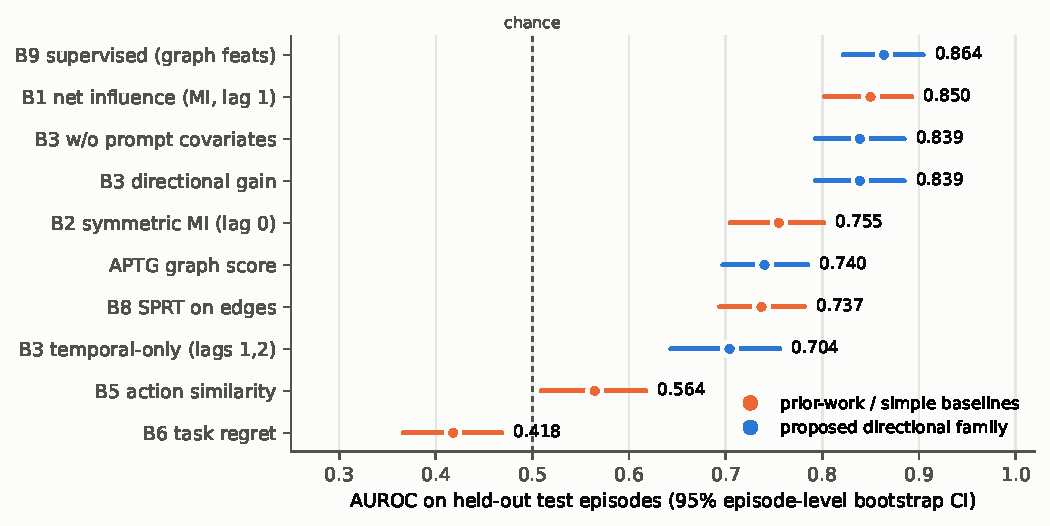
\includegraphics[width=.64\linewidth]{figs/fig_auroc.pdf}\caption{AUROC with 95\% CIs. Blue: the directional family (including B9, which uses the graph features); orange: prior-work and simple baselines.}\label{fig:auroc}\end{figure}
\textbf{H1 (directional vs.\ symmetric and net influence): not supported.} The pre-registered rule required the directional score to beat both B2 and B1; it beats B2 but is significantly worse than B1 on TPR, so we make no directional-novelty claim. B3 exceeds B2: $\Delta$AUROC \dAurocBthreeBtwo{} [\dAurocBthreeBtwoLo, \dAurocBthreeBtwoHi]. Against lag-1 net influence B1 the AUROC difference is inconclusive (\dAurocBthreeBone{} [\dAurocBthreeBoneLo, \dAurocBthreeBoneHi]) and B1 has the higher TPR (\dTprBthreeBone{} [\dTprBthreeBoneLo, \dTprBthreeBoneHi]). So the \emph{combined} same-round-and-lagged statistic is supported against symmetric MI only. The strictly lagged statistic is not: B3-temporal reaches \auroctestBtemp{} against \auroctestBtwo{} for B2 ($\Delta$AUROC \dAurocBtempBtwo{} [\dAurocBtempBtwoLo, \dAurocBtempBtwoHi], inconclusive), and the same-round term is what recovers complementary pairs (Table~\ref{tab:mech}). Realised test FPRs at the shared 5\% validation target differ (B1 0.067, B3 0.043, APTG 0.037, B8 0.020), so TPR comparisons favour detectors with higher realised FPR (AUROC does not depend on thresholds), and the TPR/FPR intervals treat the validation threshold as fixed and are somewhat too narrow.
\textbf{Mechanism specificity.} Table~\ref{tab:mech} and Fig.~\ref{fig:mech} show that no detector covers all four mechanisms. B1 is perfect on leader--follower and hidden-channel but nearly blind to complementary pairs (same-round, negative association); B2 is the reverse. B3 covers complementary, leader--follower and alternating at 0.68--0.72 but not the parity-coded hidden channel (0.10): a monotone logistic model on numeric lags cannot represent parity, whereas plug-in MI is nonparametric. B3-temporal (lags $1,2$) loses complementary pairs, confirming that simultaneous-move dependence is contemporaneous rather than lagged and directional.
\begin{table}[t]\centering\small\resizebox{\linewidth}{!}{\begin{tabular}{lcccc}
\toprule
Detector & complementary & leader-follower & alternating$^\dagger$ & hidden-channel$^\dagger$ \\
\midrule
B1 net influence (MI, lag 1) & 0.07 & 1.00 & 0.80 & 1.00 \\
B2 symmetric MI (lag 0) & 1.00 & 0.07 & 0.65 & 0.07 \\
B5 action similarity & 0.25 & 0.15 & 0.00 & 0.03 \\
B6 task regret & 0.05 & 0.03 & 0.03 & 0.00 \\
B8 SPRT on edges & 0.57 & 0.57 & 0.30 & 0.00 \\
B3 directional gain & 0.72 & 0.68 & 0.72 & 0.10 \\
B3 temporal-only (lags 1,2) & 0.07 & 0.82 & 0.70 & 0.07 \\
B3 w/o prompt covariates & 0.72 & 0.68 & 0.72 & 0.10 \\
APTG graph score & 0.78 & 0.68 & 0.47 & 0.00 \\
B9 supervised (graph feats) & 0.85 & 0.70 & 0.85 & 0.12 \\
\bottomrule
\end{tabular}}\caption{TPR at the validation-tuned 5\%-FPR threshold by mechanism (test). $^\dagger$Held out of all fits.}\label{tab:mech}\end{table}
\begin{figure}[t]\centering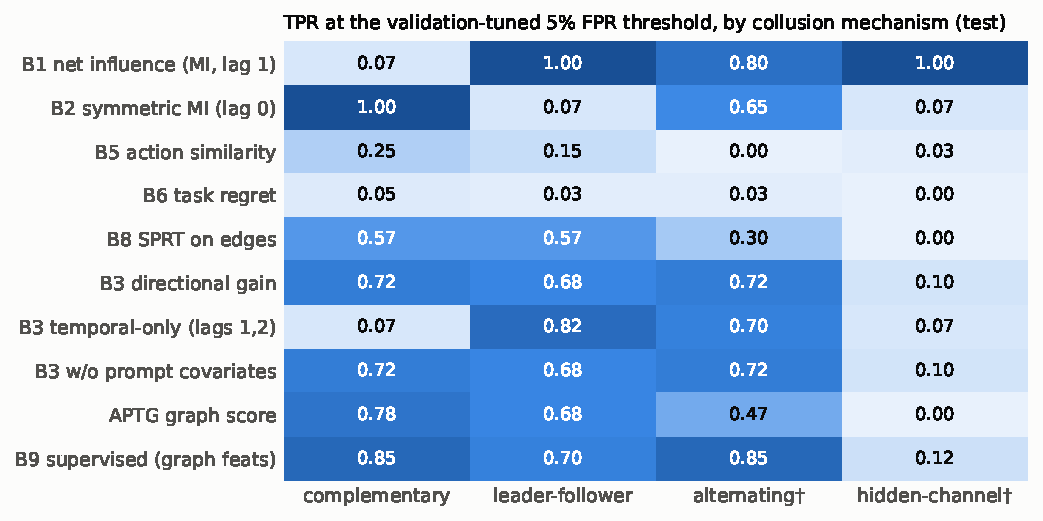
\includegraphics[width=.62\linewidth]{figs/fig_mechanism.pdf}\caption{Detector $\times$ mechanism TPR (same data as Table~\ref{tab:mech}).}\label{fig:mech}\end{figure}
\textbf{H2 (prompt conditioning).} \emph{Inconclusive.} B3 and B3-noprompt are identical, because prompt covariates are constant within an episode and our per-episode estimator therefore cannot use them. The relevant safety evidence is Table~\ref{tab:neg}: no detector shows a clear false-alarm rise under unilateral (C1/C2), common (C3) or benign-shift (C6) conditions or on shared-model and benign-adaptation negatives, with FPRs mostly near the nominal 5\%. The highest perturbation cells are B2 on C1 (0.15, i.e.\ 9/60 episodes) and B6 on C1 (0.12), and B1 is already at 0.13 on clean C0; with 60 episodes per cell (binomial half-width up to $\pm$0.09) we cannot exclude a modest increase.
\begin{table}[t]\centering\small\resizebox{\linewidth}{!}{\begin{tabular}{lccccccc}
\toprule
Detector & C0 & C1 (A pert.) & C2 (B pert.) & C3 (both) & C6 (benign shift) & benign adapt. & shared model \\
\midrule
B1 net influence (MI, lag 1) & 0.13 & 0.02 & 0.08 & 0.07 & 0.03 & 0.07 & 0.05 \\
B2 symmetric MI (lag 0) & 0.05 & 0.15 & 0.03 & 0.02 & 0.05 & 0.07 & 0.06 \\
B5 action similarity & 0.07 & 0.05 & 0.05 & 0.05 & 0.07 & 0.08 & 0.06 \\
B6 task regret & 0.07 & 0.12 & 0.08 & 0.02 & 0.03 & 0.05 & 0.06 \\
B8 SPRT on edges & 0.05 & 0.00 & 0.03 & 0.00 & 0.02 & 0.01 & 0.02 \\
B3 directional gain & 0.08 & 0.02 & 0.05 & 0.00 & 0.07 & 0.02 & 0.05 \\
B3 temporal-only (lags 1,2) & 0.13 & 0.07 & 0.07 & 0.02 & 0.02 & 0.06 & 0.04 \\
B3 w/o prompt covariates & 0.08 & 0.02 & 0.05 & 0.00 & 0.07 & 0.02 & 0.05 \\
APTG graph score & 0.07 & 0.03 & 0.05 & 0.02 & 0.02 & 0.05 & 0.03 \\
B9 supervised (graph feats) & 0.10 & 0.08 & 0.03 & 0.05 & 0.08 & 0.07 & 0.08 \\
\bottomrule
\end{tabular}}\caption{FPR at the validation-tuned threshold on each negative type (test).}\label{tab:neg}\end{table}
\textbf{H3 (temporal graph features).} \emph{Not supported.} The APTG score is below B3 (\dAurocAPTGBthree{} [\dAurocAPTGBthreeLo, \dAurocAPTGBthreeHi]); with $T{=}40$ there are only three 20-step windows, each too short for reliable per-window significance. The supervised B9 on the same features (\auroctestBnine{}) outperforms APTG by \dAurocBnineAPTG{} [\dAurocBnineAPTGLo, \dAurocBnineAPTGHi], so the features contain signal that the hand-built score discards; B9 inherits the hidden-channel blind spot (Table~\ref{tab:mech}). The SPRT stream (B8) rejects the null on \bEightPos{} of collusive and \bEightNeg{} of non-collusive test episodes, typically after window \bEightStop{}.
\begin{table}[t]\centering\small\resizebox{\linewidth}{!}{\begin{tabular}{lcc}
\toprule
Comparison (A $-$ B) & $\Delta$AUROC [95\% CI] & $\Delta$TPR [95\% CI] \\
\midrule
B3 directional gain $-$ B2 symmetric MI & 0.084 [0.031, 0.139] & 0.106 [0.018, 0.197] \\
B3 directional gain $-$ B1 net influence & -0.011 [-0.077, 0.057] & -0.162 [-0.267, -0.060] \\
APTG graph score $-$ B2 symmetric MI & -0.015 [-0.074, 0.045] & 0.031 [-0.059, 0.122] \\
APTG graph score $-$ B3 directional gain & -0.099 [-0.138, -0.058] & -0.075 [-0.130, -0.029] \\
B3 temporal-only $-$ B2 symmetric MI & -0.051 [-0.124, 0.024] & -0.031 [-0.150, 0.084] \\
B3 directional gain $-$ B3 w/o prompt covariates & 0.000 [0.000, 0.000] & 0.000 [0.000, 0.000] \\
APTG graph score $-$ B1 net influence & -0.110 [-0.175, -0.040] & -0.237 [-0.344, -0.129] \\
B9 supervised $-$ APTG graph score & 0.124 [0.084, 0.161] & 0.150 [0.095, 0.215] \\
\bottomrule
\end{tabular}}\caption{Paired episode-bootstrap differences on identical test episodes (TPR at each detector's own validation threshold).}\label{tab:paired}\end{table}
\textbf{H5 (robustness): not supported.} The drop in TPR from clean collusion to the held-out prompt family (C4 to OOD, 80 vs.\ 80 episodes) is $-0.10$ [$-0.25$, $0.05$] for APTG (no drop), against $0.01$ [$-0.11$, $0.15$] for B1, $0.11$ [$-0.04$, $0.26$] for B2 and $0.04$ [$-0.08$, $0.14$] for B5; APTG's drop is smaller than B2's (difference $-0.21$ [$-0.40$, $-0.03$]) but not clearly smaller than B1's or B5's. The drop from seen to held-out mechanisms (C4, 40 vs.\ 40) is $0.35$ [$0.15$, $0.55$] for APTG against $-0.38$ [$-0.55$, $-0.20$] for B1, i.e.\ APTG degrades \emph{more} than B1 (difference $0.73$ [$0.48$, $1.00$]) and not clearly differently from B2 ($0.23$ [$-0.03$, $0.50$]) or B5 ($0.05$ [$-0.23$, $0.33$]). Since the rule required a smaller drop than B1, B2 and B5, H5 fails. These contrasts were computed after review with \texttt{experiments/h5\_bootstrap.py} (independent episode-level bootstraps, 2000 resamples, validation thresholds fixed), not in the original scoring stage. Table~\ref{tab:robust} reports TPR on clean collusion (C4), collusion with a unilateral perturbation (C5) and a held-out prompt family (OOD). Because the baseline gate is inactive, the held-out family is never flagged out-of-calibration, so these columns measure a distribution shift on an ungated detector, not calibration-aware robustness. Directional detectors do not collapse under it; B6 (task regret) is below chance and its OOD FPR is \fproodBsix{} because family-level price shifts move payoffs without any dependence between agents. In this game scripted coordination does not raise the coalition's own payoff, so outcome-based evidence is weak by construction.
\begin{table}[t]\centering\small\resizebox{\linewidth}{!}{\begin{tabular}{lcccc}
\toprule
Detector & TPR clean (C4) & TPR + unilateral pert. (C5) & TPR held-out family (OOD) & OOD FPR \\
\midrule
B1 net influence (MI, lag 1) & 0.74 & 0.70 & 0.72 & 0.07 \\
B2 symmetric MI (lag 0) & 0.49 & 0.41 & 0.38 & 0.05 \\
B5 action similarity & 0.17 & 0.04 & 0.14 & 0.09 \\
B6 task regret & 0.04 & 0.01 & 0.45 & 0.68 \\
B8 SPRT on edges & 0.31 & 0.41 & 0.42 & 0.01 \\
B3 directional gain & 0.50 & 0.61 & 0.59 & 0.05 \\
B3 temporal-only (lags 1,2) & 0.44 & 0.40 & 0.51 & 0.09 \\
B3 w/o prompt covariates & 0.50 & 0.61 & 0.59 & 0.05 \\
APTG graph score & 0.45 & 0.51 & 0.55 & 0.05 \\
B9 supervised (graph feats) & 0.59 & 0.68 & 0.64 & 0.05 \\
\bottomrule
\end{tabular}}\caption{Robustness: TPR under unilateral perturbation (C5) and held-out prompt family; last column is FPR on OOD negatives.}\label{tab:robust}\end{table}
\textbf{H4 (RL investigator).} \emph{Weakly supported in its literal form, and not a contribution of learning.} At matched FPR ($\le0.05$ on validation, selected reward $C_{FP}{=}\rlSelCFP$, $c_{obs}{=}\rlSelCObs$) the PPO investigator decides after the first window, with test TPR \rlPpotesttpr{}, FPR \rlPpotestfpr{}, delay \rlPpotestdelay{} steps and observation cost \rlPpotestcost{}, against \rlThrtesttpr{}/\rlThrtestfpr{}/\rlThrtestdelay{}/\rlThrtestcost{} for the fixed threshold and \rlSprttesttpr{}/\rlSprttestfpr{}/\rlSprttestdelay{}/\rlSprttestcost{} for SPRT (Table~\ref{tab:rl}); so delay and cost are lower, as H4 literally requires, but recall is lower than the fixed threshold. The three PPO seeds converged to the same deterministic policy (sd $=0$), and it coincides on every split with a hand-written ``flag iff the first window has a significant edge'' rule that we added post hoc (test TPR \rlFwtesttpr{}, FPR \rlFwtestfpr{}); that rule loses \rlFwDiff{} TPR [\rlFwDiffLo, \rlFwDiffHi] to the fixed threshold. A high false-positive cost makes PPO never alert (\rlNeverAlertCfgs{} of 9 reward settings yield TPR 0). Delay is measured among true positives and the fixed threshold always sees all three windows, so PPO's lower delay and cost follow mechanically from deciding after one window; selection of the reward setting and the comparator thresholds used validation episodes from seen mechanisms only (a first selection on all validation positives chose the same settings and gave identical test numbers); the held-out mechanisms enter only the test and OOD evaluation. Following our decision rule, we report no evidence that RL adds value beyond simple rules in this setting; with three windows per episode there is little sequential structure to learn.
\begin{table}[t]\centering\small\begin{tabular}{lcccc}
\toprule
Investigator (test) & TPR & FPR & delay (steps) & cost \\
\midrule
Fixed threshold & 0.47 & 0.03 & 40.0 & 3.00 \\
SPRT & 0.36 & 0.02 & 32.1 & 2.89 \\
Uncertainty-driven & 0.37 & 0.03 & 20.0 & 3.27 \\
PPO (mean$\pm$sd, 3 seeds) & 0.37$\pm$0.00 & 0.03$\pm$0.00 & 20.0 & 1.00 \\
\bottomrule
\end{tabular}\caption{Investigators on test episodes at matched FPR $\le 0.05$ (thresholds and rewards selected on validation). Delay is the time step of the last window seen at alert; cost counts observe steps plus $2.5\times$ inspections.}\label{tab:rl}\end{table}

\begin{table}[t]\centering\small\begin{tabular}{lcccc}
\toprule
Condition & seat 0 & seat 1 & seat 2 & episodes \\
\midrule
C0 clean & 0.93 & 0.78 & 0.78 & 6 \\
C1 seat-0 perturbed & 1.97 & 0.57 & 0.45 & 6 \\
C3 all perturbed & 4.00 & 4.00 & 4.00 & 6 \\
C4L seats 0,1 told to coordinate & 2.68 & 2.82 & 1.88 & 6 \\
\bottomrule
\end{tabular}\caption{Haiku pilot: mean chosen price level per seat and condition ($T{=}10$).}\label{tab:pilot}\end{table}
\textbf{Follow-up: union of dependence statistics (exploratory, not pre-registered).} Because no single statistic covered all mechanisms, we tested the union suggested by Table~\ref{tab:mech} using the design in \texttt{FOLLOWUP\_PREREG.md}: each component is converted to a robust $z$ against training negatives and the union score is the maximum $z$, thresholded once at 5\% FPR on validation negatives (one run, no tuning). We added B4, a nonparametric lagged conditional MI $I(a_i^{t-1};a_j^t\mid a_j^{t-1})$ with a shuffle-null correction, to test the review's suggestion of a nonparametric directional component. The union U3 of B1, B2 and B3 reaches AUROC \,0.990 [0.981, 0.996] and TPR 0.950 at realised FPR 0.057, against B1's 0.850 and 0.719 (paired $\Delta$AUROC 0.140 [0.098, 0.187]; $\Delta$TPR 0.231 [0.158, 0.308]), and every mechanism is detected at 0.80 or higher (Table~\ref{tab:union}). On the held-out prompt family it keeps TPR 0.938 at FPR 0.067. Its FPR on perturbation and benign negatives stays between 0.03 and 0.07 (C1/C2 0.07), so we see no clear false-alarm cost, within the limits of 60 episodes per cell. B4 alone is weaker than B1 (AUROC 0.717; $\Delta$ vs.\ B1 $-0.133$ [$-0.186$, $-0.081$]) and, as a lag-1 statistic, misses complementary and alternating pairs; adding it to U3 changes nothing (U4$-$U3 $\Delta$AUROC $-0.003$). An all-nonparametric union (B1, B2, B4) performs almost as well (AUROC 0.983, TPR 0.925, FPR 0.053), so the gain comes from covering different dependence types rather than from the parametric gain. Caveats: the follow-up was specified after the main results were known, the mechanisms are our own scripted constructions, and the components were chosen knowing which mechanisms they cover, so this is evidence that coverage is complementary in this simulator, not that a union generalises to unseen coordination.
\begin{table}[t]\centering\small\resizebox{\linewidth}{!}{\begin{tabular}{lcccccccc}
\toprule
Detector & AUROC [95\% CI] & TPR & FPR & Compl. & Lead--fol. & Altern.$^\dagger$ & Hidden$^\dagger$ \\
\midrule
B1 net influence & 0.850 [0.803, 0.892] & 0.719 & 0.067 & 0.07 & 1.00 & 0.80 & 1.00 \\
B2 symmetric MI & 0.755 [0.705, 0.801] & 0.450 & 0.060 & 1.00 & 0.07 & 0.65 & 0.07 \\
B3 directional gain & 0.839 [0.793, 0.885] & 0.556 & 0.043 & 0.72 & 0.68 & 0.72 & 0.10 \\
B4 nonparametric lagged CMI & 0.717 [0.665, 0.771] & 0.450 & 0.053 & 0.00 & 1.00 & 0.05 & 0.75 \\
\midrule
U3 = max-z(B1,B2,B3) & 0.990 [0.981, 0.996] & 0.950 & 0.057 & 1.00 & 1.00 & 0.80 & 1.00 \\
U4 = max-z(B1,B2,B3,B4) & 0.987 [0.976, 0.994] & 0.944 & 0.067 & 1.00 & 1.00 & 0.78 & 1.00 \\
Unp = max-z(B1,B2,B4) & 0.983 [0.968, 0.992] & 0.925 & 0.053 & 1.00 & 1.00 & 0.70 & 1.00 \\
\bottomrule
\end{tabular}}\caption{Follow-up: single statistics and max-$z$ unions on the test split (460 episodes). TPR/FPR at the 5\%-FPR validation threshold; right columns are per-mechanism TPR. $^\dagger$Held out of all fits.}\label{tab:union}\end{table}
\textbf{Haiku pilot.} \pilotInvalid{} of \pilotDecisions{} responses were invalid. The manipulation check passes: in C1 the perturbed seat averages \pilotCOnePertMean{} against \pilotCOnePartnerMean{} for its unperturbed partner (clean seats $\approx$ \pilotMeanCZeroSeatOne{}), and in C3 every seat prices at 4. Telling seats 0,1 to keep both profits high lifts their mean price to \pilotCoordMean{} against \pilotCleanMean{} in C0 (one-sided Mann--Whitney $p{=}\pilotMWp{}$, 6 vs.\ 6 episodes), with the outsider also higher than in C0 (Table~\ref{tab:pilot}). With $T{=}10$ the windowed detectors do not apply; the pilot is descriptive only.

\section{Discussion and Limitations}
\textbf{Implications.} For an auditor, the practical message is that dependence statistics are \emph{mechanism-specific}: a lagged-MI monitor, a same-round MI monitor and a parametric directional monitor each cover a different part of the space, and a parity-coded channel needs a nonparametric statistic. A union of detectors is the natural response, and the exploratory follow-up above supports it (U3 AUROC 0.990 against 0.850 for the best single statistic), but it was specified after the main results and needs testing on mechanisms we did not script. Reassuringly, unilateral steering of one agent did not produce a clear rise in false alarms in any detector in our simulator, though the cells are small.
\textbf{Prompt conditioning, still to be tested.} The motivating distinction is between an \emph{individual policy shift} (an instruction changes one agent's action distribution) and \emph{new inter-agent dependence}; the two must not be conflated. A faithful test needs a baseline $P(A_{i,t}\mid H_i^{t-1},C_t,M_i,P_i,\tau_i)$ over the agent's own history, public context, model or endpoint identity $M_i$, instruction family $P_i$ and decoding settings $\tau_i$. Because prompt conditions are constant within an episode, it must be estimated \emph{across} episodes (pooled or hierarchical) and then compared with matched non-collusive controls under unilateral perturbation. We write the model only to define the extension; it is untested here, and writing it down is not a substitute for the experiment.
\textbf{Limitations.} (1) \emph{Simulator evidence.} The scripted mechanisms are our own construction and share assumptions with the detectors; a single environment, three agents, $T{=}40$; no DCOP/task-regret environment. (2) \emph{Scale.} Fewer seeds than the planned 100/cell (train 10, val 12, test 20, OOD 10), so CIs are wide, and 30 permutations per edge give coarse $p$-values. (3) \emph{Prompt conditioning is not tested.} The calibration baseline is implemented but not wired into the detectors, so every episode counts as calibrated and the out-of-calibration gate never fires; the prompt covariates in the estimator are constant within an episode, making the ablation vacuous. A pooled estimator across episodes with a per-family reference is needed. (4) \emph{Graph score.} Three windows per episode is too few to test temporal motifs; H3 is not supported \emph{at this scale}, not refuted in general. (5) \emph{RL.} Few windows, a small training set and 20k PPO steps; results say little about RL for audit in general. (6) \emph{LLM pilot.} Haiku sellers were driven as subagents, without temperature control, and a subagent answers the prompts of one seat across episodes, so independence between agents is approximate; 6 episodes per condition. (7) \emph{Collusion is behavioural.} Scripted coordination does not raise coalition payoff here, so we claim operational evidence of coordination, not intent or harm. (8) Edges are predictive, not causal. (9) \emph{Planned but not run.} Of the pre-registered secondary outcomes and ablations we did not run: calibration (Brier/ECE), group localization, detection delay for any detector other than B8 and the RL investigators, the LLM-judge baseline, and the no-temporal-motif and no-regret-feature ablations; the prompt-conditioned ablation is vacuous (H2). (10) \emph{Statistical details.} Block-permutation draws use the same seeds in every episode, so $p$-values are correlated across episodes; max-statistic draws are independent per edge (conservative: on 60 independent-episode edge tests the single-edge rejection rate at nominal 0.05 was 0.017); cross-fitted folds are blocked and purged but not causal. (10) \emph{Unplanned exclusion.} One validation negative (\texttt{benign\_adaptation-C0-s61-f1}) has no window record, so B8 scores it 0 and the RL validation set has 275 episodes.
\textbf{Future work.} A pooled prompt-conditioned baseline evaluated against matched unilateral-perturbation controls; a union tested on learned (not scripted) collusion and on mechanisms not known to the designers; a strictly lagged directional detector with a parity-capable (nonparametric) model class; a properly powered comparison of the RL investigator with simple sequential rules; longer episodes and denser windows; a DCOP environment with real task regret; multiple model families; more LLM episodes through an API with controlled sampling.

\section{Conclusion}
In a pre-registered, sprint-scale test of the APTG-RL design, a combined same-round-and-lagged directional gain improved on symmetric mutual information but not on lag-1 net influence (and its strictly lagged part showed no clear improvement on it), the detectors proved complementary rather than ranked (an exploratory max-$z$ union of three of them detected every mechanism, AUROC 0.990), the graph score and RL investigator added no measurable value, and unilateral prompt steering did not clearly raise false alarms. The most actionable lessons are about coverage (no single dependence statistic sees every coordination pattern) and about evaluation design (hold out mechanisms, report negative controls and deviations).

\paragraph{Code and Data.}
Code, configs, seeds, pre-registration and raw results: \url{https://github.com/chinchoooo/COLDER} (repository \texttt{COLDER}). The scripted data are regenerable from seeds; the Haiku pilot logs are in \texttt{results/llm/}. All code was written during the sprint; the only pre-existing material is the author's two APTG-RL proposal documents (no code, no results).
\paragraph{Author Contributions.}
A.K.\ conceived the design, specified the experiments and wrote the report; code and drafting were produced with AI assistance (below) under the author's direction.

\bibliographystyle{plainnat}
\bibliography{refs}

\appendix
\section{Limitations and Dual-Use / Ethical Considerations}\label{app:ethics}
\textbf{What the results establish.} In one synthetic pricing game with scripted coordination, on held-out simulated episodes, specific dependence statistics detect specific coordination patterns at a stated false-alarm rate, and unilateral steering of one agent did not clearly raise those false-alarm rates (cells of 60 episodes). A small Haiku pilot shows that instructions move prices.
\textbf{What they do not establish.} They do not show that these detectors work on real deployed agents, on learned (rather than scripted) collusion, on other games, or against agents that adapt to the monitor. They say nothing about intent: a detector alarm is evidence of statistical coordination under explicit rules, not proof of malicious behaviour, and false accusations have real costs (the investigator's reward weights $C_{FP}$ are a policy choice). Edges are predictive, not causal. Power is limited (Section~5).
\textbf{Dual-use.} The testbed includes a hidden-channel mechanism that evades two of our detectors (B3, APTG). This is a closed toy protocol (a parity code on a five-level action) and is described because the failure is an audit finding; however, a reader could learn that parity-style codes are invisible to monotone parametric monitors. We mitigate by keeping the protocol toy-scale, reporting that a nonparametric MI statistic detects it (B1: 1.00), not releasing any optimiser for evasion, and recommending nonparametric statistics in monitors. The LLM pilot includes a prompt that tells agents to keep both profits high; in a real market this would be price coordination, which is illegal in many jurisdictions. It is used only in a toy game with fictional sellers; no real market data, personal data or real endpoints were used.
\textbf{Responsible use.} Detector outputs should be treated as triage evidence for human review, reported with uncertainty, and never as automatic grounds for sanctions.

\section{Deviations from the Pre-registration}\label{app:dev}
All were decided before any test, OOD or pilot detector evaluation, from training-seed smoke tests (full log: \texttt{DEVIATIONS.md}). (1) Westfall--Young max-statistic control replaces BH in the windowed graph: with $\le 200$ permutations the smallest attainable $p$ is $1/(n{+}1)$ and BH over 6 pairs needs $p\le q/6\approx0.0083$, so a single strong edge could never be rejected (a smoke test on a clear leader--follower episode scored 0). (2) Window 20/stride 10 instead of 10/5 (training smoke: leader--follower persistence 0.50 vs.\ 0.26). (3) 30 permutations per edge. (4) Fewer seeds (Section~5). (5) B3 takes the maximum over all six ordered pairs (the detector does not know the coalition); B3-temporal and B3-noprompt were added. (6) The no-prompt ablation is applied to B3 only. (7) The RL reward grid and comparator thresholds were first selected on all validation positives, including the held-out mechanisms, contrary to the plan; we repeated the selection on seen mechanisms only (227 validation episodes) and report that version. The selected settings and every test number were identical. (8) \emph{Follow-up (not in the plan):} the union experiment follows \texttt{FOLLOWUP\_PREREG.md}, which was written before the follow-up scripts were run but, unlike \texttt{PREREG.md}, was committed together with its results, so its timing is not independently verifiable. (9) \emph{LLM pilot redesign:} the first pilot (perturbation: ``undercut aggressively'') failed its manipulation check, since Haiku already prices at the low level, and produced near-identical episodes within a condition; it was discarded after two rounds and replaced by a misleading task detail plus neutral role descriptions (``a shop owner'', etc.). No detector had been run on either pilot.

\section{LLM pilot prompt}\label{app:prompt}
\small\noindent Each decision prompt reads: \emph{``You are seller $k$, <role>, in a repeated market game with 3 sellers (numbered 0, 1, 2) over 10 rounds. Each round every seller simultaneously picks an integer price level from 0 to 4. The seller(s) with the lowest price take the whole market; ties split it equally. Your payoff each round = your price level $\times$ your market share (so a high price only pays if you win the market). Your goal: maximize your own total payoff.''} followed, as applicable, by the perturbation (``Market note (from a trade newsletter): in this market customers read a high price as a quality signal and tend to buy from the highest-priced seller, so a price of 3 or 4 attracts the most customers.'') or the coordination instruction (``You and seller $m$ want to keep both of your profits high over the whole game. You may not message each other, but choose prices you think will help you both.''), the history of rounds (all three prices and the seller's own payoff), and the format request \texttt{ACTION: <n>}. Prompts never contain other agents' prompts or labels.

\section*{LLM Usage Statement}
Claude (Anthropic) was used throughout: to help design and critique the experiments, to write and debug the code (implementation was delegated to Claude subagents and reviewed), to run the Claude Haiku~4.5 agents of the pilot, and to draft this report. All numbers in the paper are generated by scripts from the committed result files; references were each checked against the publisher or preprint page (or Crossref) by the author's assistant; one reference from the original proposal that could not be verified was dropped. The author is responsible for all claims.
\end{document}
